\documentclass{trax}

\title{TRAX: Transactional, Crash-Recoverable, and\\ Ownership-Separated Code Policies for Real-World Robotics}
\runningtitle{TRAX: Transactional, Crash-Recoverable, and Ownership-Separated Code Policies}
\traxheaderleft{Tiwater}
\traxdate{November 2026}
\traxauthors{Tiwater}
\traxaffil{\href{mailto:research@tiwater.com}{\texttt{research@tiwater.com}}}
\traxlinks{%
  Project Page: \url{https://tiwater.github.io/trax/} \qquad
  Code \& Receipts: \url{https://github.com/tiwater/trax}
}

\begin{document}

\makeacademictitle

% --- Page-1 Hero Teaser Figure (Classic DeepSeek-R1 / RAX Academic Cover) ---
\begin{figure}[!ht]
\centering
% Row 1: 3-Panel PBR Workstation Photos with subtle caption bars
\begin{tikzpicture}
  \node[inner sep=0pt] (p1) at (0,0) {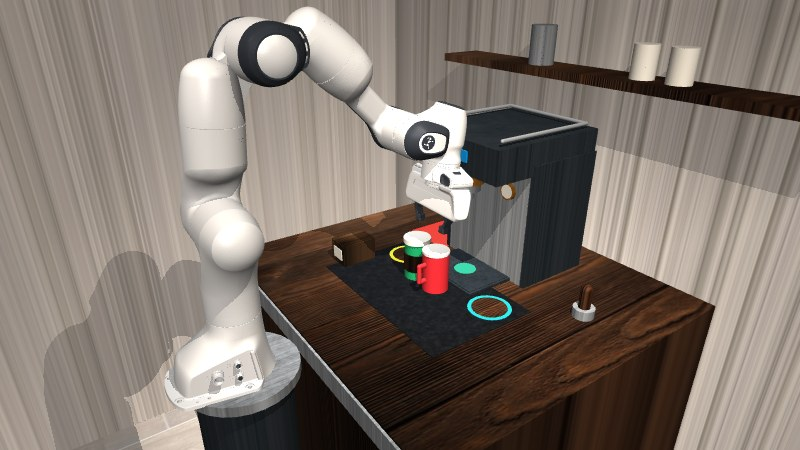
\includegraphics[width=0.323\linewidth]{figures/panda_pbr_overview.jpg}};
  \node[inner sep=0pt, right=0.014\linewidth of p1] (p2) {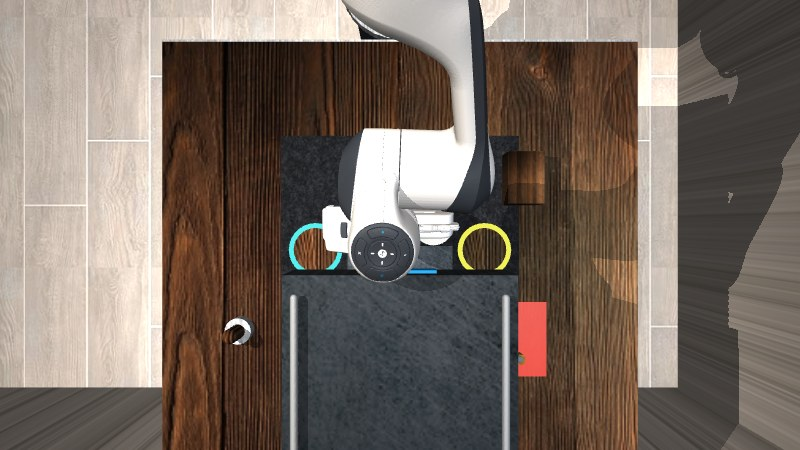
\includegraphics[width=0.323\linewidth]{figures/panda_pbr_overhead.jpg}};
  \node[inner sep=0pt, right=0.014\linewidth of p2] (p3) {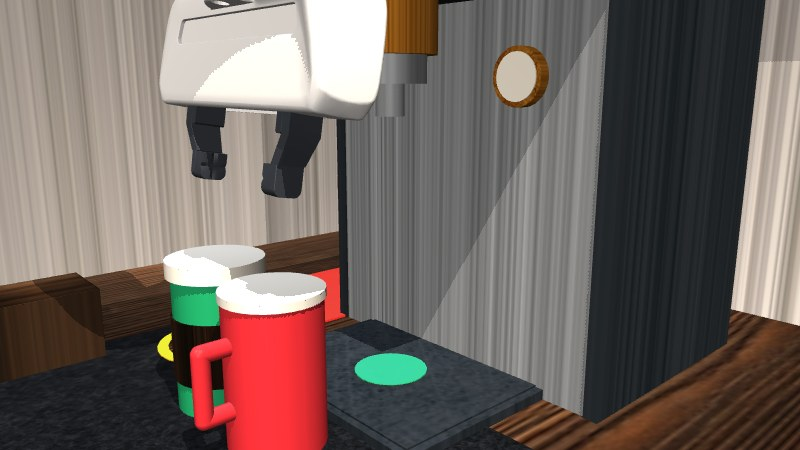
\includegraphics[width=0.323\linewidth]{figures/panda_pbr_spout.jpg}};
  \foreach \nd/\lbl in {p1/{(a) 7-DOF Panda Caf\'e Cell}, p2/{(b) Overhead \& Sim2Sim DR}, p3/{(c) Spout Alignment \& Interlocks}} {
    \fill[black, fill opacity=0.62] (\nd.south west) rectangle ([yshift=13pt]\nd.south east);
    \node[anchor=west, text=white, font=\sffamily\scriptsize] at ([xshift=4pt,yshift=6.5pt]\nd.south west) {\lbl};
  }
\end{tikzpicture}

\vspace{5pt}

% Row 2: 3 Compact Vector Summary Bar Charts
\resizebox{\linewidth}{!}{%
\begin{tikzpicture}[font=\sffamily\scriptsize]
  % Helper style
  \tikzset{
    panel/.style={draw=traxrule, fill=traxbg, rounded corners=2pt, line width=0.5pt},
    ptitle/.style={font=\sffamily\scriptsize\bfseries, text=traxink, anchor=west},
    psub/.style={font=\sffamily\tiny, text=traxmuted, anchor=west},
    lbl/.style={font=\sffamily\tiny, text=traxink, anchor=east},
    val/.style={font=\sffamily\tiny\bfseries, text=traxink, anchor=west},
    valm/.style={font=\sffamily\tiny, text=traxmuted, anchor=west}
  }

  % Panel (d): Commercial Workstations
  \draw[panel] (0,0) rectangle (5.15,2.55);
  \node[ptitle] at (0.16,2.30) {(d) Commercial Safety \& Transfer};
  \node[psub]   at (0.16,2.04) {MuJoCo + recorded\_data shadow (0 dup / 0 false act)};
  % Bars: x=1.75 .. 4.30 (width 2.55 = 100%)
  \foreach \y/\name/\pct/\hi/\txt in {
    1.62/{CafeBench v2}/1.00/1/{100\%},
    1.30/{Strongest Base.}/0.767/0/{76.7\%},
    0.88/{Sim2Sim ($\le$5)}/0.95/1/{95.0\%},
    0.56/{SimEX-Prot.}/0.80/0/{80.0\%},
    0.18/{Combo v3 (+62\%)}/1.00/1/{100\%}
  }{
    \node[lbl] at (1.70,\y+0.09) {\name};
    \ifnum\hi=1
      \fill[traxaccent, rounded corners=1pt] (1.76,\y) rectangle ({1.76+2.50*\pct},\y+0.19);
      \node[val] at ({1.82+2.50*\pct},\y+0.09) {\txt};
    \else
      \fill[traxrule, rounded corners=1pt] (1.76,\y) rectangle ({1.76+2.50*\pct},\y+0.19);
      \node[valm] at ({1.82+2.50*\pct},\y+0.09) {\txt};
    \fi
  }

  % Panel (e): Zero-Leakage Robosuite v4
  \begin{scope}[xshift=5.35cm]
    \draw[panel] (0,0) rectangle (5.15,2.55);
    \node[ptitle] at (0.16,2.30) {(e) Zero-Leakage Robosuite v4 ($n{=}80$)};
    \node[psub]   at (0.16,2.04) {4 tasks $\times$ 20 seeds; 0 eval LLM, 23$\times$ faster p95};
    \foreach \y/\name/\pct/\hi/\txt in {
      1.62/{TRAX (Ours)}/0.900/1/{90.0\%},
      1.26/{CaP-X (Online)}/0.838/0/{83.8\%},
      0.90/{SimEX-Prot.}/0.637/0/{63.7\%},
      0.54/{ASPIRE-Prot.}/0.613/0/{61.3\%},
      0.18/{Zero-Shot}/0.250/0/{25.0\%}
    }{
      \node[lbl] at (1.70,\y+0.09) {\name};
      \ifnum\hi=1
        \fill[traxaccent, rounded corners=1pt] (1.76,\y) rectangle ({1.76+2.50*\pct},\y+0.19);
        \node[val] at ({1.82+2.50*\pct},\y+0.09) {\txt};
      \else
        \fill[traxrule, rounded corners=1pt] (1.76,\y) rectangle ({1.76+2.50*\pct},\y+0.19);
        \node[valm] at ({1.82+2.50*\pct},\y+0.09) {\txt};
      \fi
    }
  \end{scope}

  % Panel (f): LIBERO-Spatial & Blind LIBERO-Object
  \begin{scope}[xshift=10.70cm]
    \draw[panel] (0,0) rectangle (5.20,2.55);
    \node[ptitle] at (0.16,2.30) {(f) LIBERO 10/10 (\texttt{host\_state\_api})};
    \node[psub]   at (0.16,2.04) {Spatial ($n{=}100$) + zero-tuning Blind Object ($n{=}100$)};
    \foreach \y/\name/\pct/\hi/\txt in {
      1.62/{Spatial: TRAX}/0.97/1/{97.0\%},
      1.28/{Spatial: ASPIRE}/0.89/0/{89.0\%},
      0.86/{Blind Obj: TRAX}/0.88/1/{88.0\%},
      0.52/{Blind Obj: SimEX}/0.82/0/{82.0\%},
      0.18/{Blind Obj: RAX-P}/0.80/0/{80.0\%}
    }{
      \node[lbl] at (1.74,\y+0.09) {\name};
      \ifnum\hi=1
        \fill[traxaccent, rounded corners=1pt] (1.80,\y) rectangle ({1.80+2.48*\pct},\y+0.19);
        \node[val] at ({1.86+2.48*\pct},\y+0.09) {\txt};
      \else
        \fill[traxrule, rounded corners=1pt] (1.80,\y) rectangle ({1.80+2.48*\pct},\y+0.19);
        \node[valm] at ({1.86+2.48*\pct},\y+0.09) {\txt};
      \fi
    }
  \end{scope}
\end{tikzpicture}}
\caption{\textbf{Overview of TRAX.} \emph{Top (a--c):} MuJoCo~3.3.0 7-DOF Franka Panda PBR caf\'e workstation (\texttt{evidence\_source=simulator}) evaluating non-idempotent crash reconciliation, Sim-to-Sim noise/DR transfer, and multi-appliance interlocks. \emph{Bottom (d--f):} Matched-backend (\texttt{gpt-6-astra}) held-out success across commercial workstations, zero-leakage Robosuite~v4 (480 rollouts), official \textsc{LIBERO-Spatial} (10/10), and a pre-registered zero-tuning blind \textsc{LIBERO-Object} generalization test (10/10), achieving \textbf{257/280 (91.8\%)} with zero task collapses across all 24 external tasks.}
\label{fig:overview}
\end{figure}

\begin{abstract}
Agentic code-as-policies systems can synthesize robot manipulation programs from natural language, yet deploying them in commercial workstations---such as espresso brewing, bagel/oven heating, and shared-arm multi-appliance fulfillment---exposes five operational failure modes left unresolved by simulation-only agents: non-idempotent appliance crashes, blurred perception-to-actuation authority, coupled self-evaluation, multi-second online LLM latency, and sequential single-appliance bottlenecks. We present \textbf{TRAX} (\emph{Transactional Robot Action eXecution}), a pure-Python-stdlib policy governance, crash reconciliation, and bounded offline evolution framework enforcing strict three-owner separation between perception (e.g., EvidenceScene), deterministic policy execution, and host actuation. Online, TRAX executes SHA-256-frozen policies inside a restricted Python AST sandbox with zero online LLM calls and an intent-before-dispatch SQLite journal enforcing query-first reconciliation. Offline, TRAX combines zero-leakage public-SDK \emph{Active Physical Probing}, closed-loop simulator calibration, multi-hypothesis \texttt{RepairScreener} with AST selective subroutine repair, zero-actuation \texttt{recorded\_data} shadow gating, decoupled independent acceptance, and contract-drift-aware executable skill toolboxes. Across five evidence-tagged tracks using a matched LLM backend (\texttt{gpt-6-astra}): TRAX achieves \textbf{30/30 (100\%, 0 duplicates)} on \textsc{CafeBench~v2} ($p{=}0.0156$ vs.\ adapted ASPIRE/CaP-X), \textbf{19/20 (95\%)} on $\le 5$-trial Sim-to-Sim adaptation, \textbf{12/12 (100\%, +62.5\% throughput)} on \textsc{CafeBench~v3} combo operations, \textbf{72/80 (90.0\%, \#1 on every task)} on zero-leakage Robosuite~v4 ($23\times$ faster $p_{95}$ than online CaP-X; $p \le 1.9{\times}10^{-5}$ vs.\ frozen baselines), \textbf{97/100 (97.0\%)} on \textsc{LIBERO-Spatial} ($p{=}0.0386$ vs.\ ASPIRE), and \textbf{88/100 (88.0\%, 0 zero-score collapses)} on pre-registered zero-tuning blind \textsc{LIBERO-Object} (exceeding matched-contract RAX-Protocol at $80/100$ and SimEX-Protocol at $82/100$, and tying ASPIRE at $90/100$, $p{=}0.824$). Physical-robot qualification remains pending; no simulation result is claimed as hardware safety approval.
\end{abstract}

\section{Introduction}
\label{sec:intro}

Code-generating robot agents have progressed rapidly from single-shot program synthesis~\cite{liang2022cap,singh2022progprompt} to closed-loop repair~\cite{schlesinger2024roborepair,ahn2025reliablecap}, standardized coding-agent benchmarks~\cite{fu2026capx}, autonomous skill discovery~\cite{lu2026aspire,enpire2026,ace2026}, simulation-integrated autoresearch (SimEX~\cite{hu2026simex}), and scalable online exploration (RAX~\cite{huang2026rax}). Despite these advances, commercial real-world workstations---such as automated espresso preparation, bagel heating, and multi-appliance combo fulfillment---remain poorly served by drop-in deployment of research agent frameworks.

Examining why recent state-of-the-art frameworks such as SimEX~\cite{hu2026simex} and RAX~\cite{huang2026rax} cannot be deployed directly in a commercial robotic cell reveals five structural gaps:
\begin{enumerate}
    \item \textbf{Non-Idempotent External Appliances and Crash Reconciliation:} A coffee brewer or high-speed oven cannot be safely retried after a network timeout, process crash, or lost acknowledgement. Retrying \texttt{start\_brew} without querying durable execution intent causes hot-liquid overflow or burnt food; conversely, blindly aborting wastes orders.
    \item \textbf{Strict Authority and Ownership Separation:} Commercial deployments integrate independent perception owners (e.g., 6-DoF scene trackers), policy orchestration, and host safety controllers owning thermal, door, and kinematic interlocks. Agents that own raw RGB-D perception pipelines or bypass host interlocks violate safety certification boundaries and risk papering over perception or device defects with fragile policy workarounds.
    \item \textbf{Decoupled Acceptance and Zero-Actuation Shadow Gating:} Model-generated code is an untrusted draft; syntax validity is not safety approval. Production rollout requires an independent acceptance evaluator distinct from the proposer, plus zero-actuation \texttt{recorded\_data} shadow checks that block false actuations on stale or ambiguous sensor frames.
    \item \textbf{Deterministic Online Latency and Bounded Onboarding Cost:} SimEX reports $\sim 3{,}360$ Stage-1 LLM calls ($21.6\,\mathrm{h}$) per task~\cite{hu2026simex}, while RAX scales to $16$--$128$ online episodes ($4.9$--$14.2\,\mathrm{h}$)~\cite{huang2026rax}. Store-level deployment requires minute-scale offline adaptation and \emph{zero} online LLM calls during service hours to avoid multi-second stall tails.
    \item \textbf{Shared-Arm Multi-Appliance Concurrency:} A single robotic arm serving both an espresso machine and an oven must pipeline idle appliance heating/brewing windows under strict host thermal/door interlocks rather than executing appliances sequentially.
\end{enumerate}

We present \textbf{TRAX} (\emph{Transactional Robot Action eXecution}), a lightweight, pure-Python-stdlib governance and closed-loop evolution framework designed specifically around these commercial constraints while absorbing the strongest compatible mechanisms from SimEX and RAX. Rather than competing with perception or low-level control stacks, TRAX defines an explicit transactional contract boundary between perception authorities, deterministic policy execution, and host actuation.

\paragraph{Evidence Scope and Provenance.} Throughout this report, we enforce a strict four-tier evidence separation: \texttt{fixture} (deterministic software contracts), \texttt{simulator} (MuJoCo~3.3.0 PBR caf\'e workstation, Robosuite~1.5.2 Panda, and optional LIBERO), \texttt{recorded\_data} (zero-actuation replay of recorded/logged perception frames), and \texttt{physical\_robot} (currently $0$ physical hardware qualification runs; explicitly future work). Every quantitative table is deterministically generated from immutable archived JSON receipts with explicit evidence tags. Archived receipts from earlier milestones retain legacy internal codename keys (\texttt{craft\_full}) without altering any numerical measurements.

Our contributions are fourfold:
\begin{enumerate}
    \item \textbf{Ownership-Separated Runtime Governance and Intent-Before-Dispatch Reconciliation (Sections~\ref{sec:formulation} and~\ref{sec:method}):} We formalize a four-layer failure attribution taxonomy (\texttt{perception} / \texttt{control} / \texttt{device} / \texttt{policy}), a restricted Python AST sandbox executing SHA-256-frozen bundles with zero online LLM calls, and a crash-recoverable SQLite command journal enforcing query-first reconciliation on non-idempotent appliance actions.
    \item \textbf{Zero-Leakage Active Physical Probing, Closed-Loop Sim Calibration, and Selective Subroutine Repair (Section~\ref{sec:method}):} We introduce task-agnostic diagnostic probes strictly over public host SDKs (zero hardcoded task constants), bounded simulator parameter calibration for physics-mismatched Sim-to-Sim adaptation, and a multi-hypothesis \texttt{RepairScreener} enhanced with AST-guided selective subroutine repair, adaptive stagnation escape, and negative-attempt memory.
    \item \textbf{Verified Executable Skill Toolbox and Commercial Operations Loop (Section~\ref{sec:method}):} We store AST-verified helper snippets paired with empirical \texttt{measured\_limits}, \texttt{regression\_case\_ids}, and automatic invalidation upon host SDK contract drift, embedded inside a Day-Shift $\to$ Nightly Evolution $\to$ Independent Acceptance $\to$ Versioned Rollback operational loop.
    \item \textbf{Reproducible Multi-Track Empirical Evaluation (Section~\ref{sec:experiments}):} Using a matched real model backend (\texttt{gpt-6-astra}) across five evaluation tracks---Day/Night Operations Loop + \textsc{CafeBench~v2}, $\le 5$-trial Sim-to-Sim Stage-2 adaptation, \textsc{CafeBench~v3} multi-appliance combo operations, zero-leakage Robosuite~v4 Panda manipulation ($480$ rollouts), and official \textsc{LIBERO-Spatial} ($10/10$) plus pre-registered zero-tuning blind \textsc{LIBERO-Object} ($10/10$)---we demonstrate statistically significant gains over adapted ASPIRE, CaP-X, SimEX, and RAX protocols while honestly archiving failed intermediate runs and remaining gaps.
\end{enumerate}

\section{Related Work and Positioning}
\label{sec:related}

\paragraph{Code-as-Policies and Closed-Loop Program Repair.} Code as Policies~\cite{liang2022cap} and ProgPrompt~\cite{singh2022progprompt} established LLM synthesis of Python robot control scripts over perception and motion primitives, later extended with 3D value maps (VoxPoser~\cite{huang2023voxposer}), relational keypoints (ReKep~\cite{huang2024rekep}), language corrections (DROC~\cite{zha2023droc}), in-context control feedback (InCoRo~\cite{zhu2024incoro}), and service-robot deployment (CodeBotler~\cite{hu2023codebotler}). RoboRepair~\cite{schlesinger2024roborepair} and Reliable-CaP~\cite{ahn2025reliablecap} introduced structured trace-driven repair and neuro-symbolic guards. However, these methods assume idempotent or stateless primitives and omit persistent intent journaling, multi-appliance interlocks, and decoupled release governance.

\paragraph{Agentic Skill Discovery, Benchmarks, and Online Exploration.} Recent frameworks scale agentic code generation through benchmarking and iterative experience: CaP-X~\cite{fu2026capx} evaluates coding agents with multi-turn online regeneration; ASPIRE~\cite{lu2026aspire} and ENPIRE~\cite{enpire2026} autonomously discover reusable skills and self-improve real-world policies; ACE-CaP-0~\cite{ace2026}, Voyager~\cite{wang2023voyager}, RoboSkill~\cite{xie2026roboskill}, AMP~\cite{chen2026amp}, and RoboClaw~\cite{li2026roboclaw} build persistent experience libraries for long-horizon manipulation. Most closely related to TRAX's offline evolution loop are \textbf{SimEX}~\cite{hu2026simex} (simulation-integrated autoresearch with iterative simulator calibration, paired code-plus-experience libraries, and $\le 5$-trial real-world adaptation) and \textbf{RAX}~\cite{huang2026rax} (scaling online exploration with selective subroutine repair, working memory of failed attempts, and backend refusal diagnostics). Table~\ref{tab:positioning} positions TRAX against these paradigms: TRAX adopts SimEX's simulator-calibrated multi-hypothesis screening and RAX's selective subroutine repair, while adding strict ownership separation, SQLite transactional reconciliation, independent acceptance, and zero-online-LLM deterministic service execution.

\begin{table}[t]
\centering
\caption{Architectural positioning of TRAX against representative code-as-policies and agentic robotics frameworks.}
\label{tab:positioning}
\small
\resizebox{\linewidth}{!}{%
\begin{tabular}{@{}lccccccc@{}}
\toprule
Framework & Ownership Boundary & Non-Idempotent Journal & Indep.\ Gate + Shadow & Online LLM Calls & Offline Budget & Multi-Appliance & Code Status \\
\midrule
CaP / ProgPrompt~\cite{liang2022cap,singh2022progprompt} & Coupled scripts & No & No & $0$ (single-shot) & $1$ call & No & Public \\
CaP-X~\cite{fu2026capx} & Benchmark harness & No & Env reward only & Multi-turn ($>0$) & Low--Med & No & Public \\
ASPIRE~\cite{lu2026aspire} & Skill library agent & No & Self-verified & $0$ (frozen skill) & Med & No & Public \\
SimEX~\cite{hu2026simex} & Unified sim/real & No & Sim replay only & $0$ (frozen code) & $\sim 3{,}360$ calls ($21.6\,\mathrm{h}$) & No & Closed \\
RAX~\cite{huang2026rax} & Agent owns RGB-D & No & Env reward only & Online episodes & $16$--$128$ eps ($4.9$--$14.2\,\mathrm{h}$) & No & Research \\
\rowcolor{traxrow}
\textbf{TRAX (Ours)} & \textbf{Strict 3-Owner} & \textbf{SQLite Query-First} & \textbf{Decoupled + 0-Act} & \textbf{0 (Frozen AST)} & \textbf{2--12 calls (mins)} & \textbf{Pipelined + Locks} & \textbf{Pure Stdlib} \\
\bottomrule
\end{tabular}}
\end{table}

\section{Problem Formulation and Ownership Boundaries}
\label{sec:formulation}

\subsection{Three-Owner Commercial Workstation Decomposition}
We model a commercial robotic cell as three strictly separated authorities:
\begin{enumerate}
    \item \textbf{Perception Owner} ($\mathcal{P}$, e.g., EvidenceScene): Produces timestamped object/appliance state observations $o_t = (\text{entities}_t, \text{conf}_t, \text{age}_t, \text{ambig}_t)$ from sensors or \texttt{recorded\_data}. TRAX never synthesizes, smooths, or invents scene geometry.
    \item \textbf{Policy Governance Owner} ($\mathcal{C}$, TRAX): Executes a frozen policy program $\pi_\theta$ inside a restricted AST sandbox, maps policy calls into durable command intents, reconciles ambiguous receipts, and manages offline evolution, acceptance gating, and version rollback.
    \item \textbf{Host Actuation Owner} ($\mathcal{H}$, e.g., \texttt{ticos-edge} or simulator host): Owns robot kinematics, appliance drivers, physical interlocks (thermal, oven door, liquid pour alignment), timeouts, and explicit status-query endpoints \texttt{query\_action\_status(idempotency\_key)}.
\end{enumerate}

\subsection{Non-Idempotent Command Lifecycle}
Partition host actions into idempotent observations/re-centerings $\mathcal{A}_{\mathrm{idem}}$ and non-idempotent physical commitments $\mathcal{A}_{\mathrm{non}}$ (e.g., \texttt{start\_coffee\_machine}, \texttt{start\_oven\_heat}). Every call $a \in \mathcal{A}_{\mathrm{non}}$ receives a deterministic key $k = \text{key}(\text{order\_id}, \text{step}, \text{attempt\_scope})$ and transitions through an explicit state machine:
\begin{equation}
    \texttt{INTENT} \xrightarrow{\;\text{dispatch}\;} \texttt{DISPATCHED} \xrightarrow{\;\text{receipt}\;} \{\texttt{SUCCEEDED},\; \texttt{FAILED},\; \texttt{UNKNOWN}\}.
\end{equation}
If a crash or timeout yields \texttt{UNKNOWN}, the policy \emph{must not} re-dispatch $a$; instead, the runtime executes a mandatory \texttt{RECONCILE} transition via $\mathcal{H}.\texttt{query\_action\_status}(k)$. Crucially, we do \emph{not} claim distributed exactly-once physical execution from a local SQLite journal alone: exact single actuation requires cooperative host-side idempotency key verification, and unresolved ambiguity fails closed into operator escalation.

\subsection{Four-Layer Failure Attribution and Evidence Taxonomy}
When an execution fails, naive code-repair agents blindly edit policy code even when the root cause is a stale camera or broken appliance. TRAX enforces four-layer attribution $\ell(e) \in \{\texttt{perception},\, \texttt{control},\, \texttt{device},\, \texttt{policy}\}$ before invoking policy repair, blocking policy edits that would mask perception or hardware faults. Every verification record carries an explicit tag $s \in \{\texttt{fixture},\, \texttt{simulator},\, \texttt{recorded\_data},\, \texttt{physical\_robot}\}$ so simulation success can never be conflated with physical safety qualification.

\section{The TRAX Architecture and Method}
\label{sec:method}

Figure~\ref{fig:architecture} illustrates the end-to-end TRAX runtime and offline evolution architecture. All core governance modules under \texttt{src/trax/} depend exclusively on the Python~3.10 standard library; physics simulators (\texttt{mujoco\_cafe\_driver.py}, \texttt{robosuite\_bench.py}, \texttt{libero\_bench.py}) are strictly isolated optional modules.

\begin{figure}[t]
\centering
\resizebox{\linewidth}{!}{%
\begin{tikzpicture}[
    font=\sffamily\footnotesize,
    zone/.style={draw=traxrule, rounded corners=3pt, line width=0.6pt, inner sep=6pt},
    card/.style={draw=traxrule, fill=white, rounded corners=2.5pt, line width=0.55pt, align=left, inner sep=5pt},
    hi/.style={draw=traxaccent, fill=traxrow, rounded corners=2.5pt, line width=0.75pt, align=left, inner sep=5pt},
    ok/.style={draw=traxgreen!55, fill=traxgreenbg, rounded corners=2.5pt, line width=0.65pt, align=left, inner sep=5pt},
    warn/.style={draw=traxamber!55, fill=traxamberbg, rounded corners=2.5pt, line width=0.65pt, align=left, inner sep=5pt},
    arr/.style={-{Latex[length=2mm]}, line width=0.75pt, color=traxmuted},
    barr/.style={-{Latex[length=2mm]}, line width=0.85pt, color=traxaccent},
    garr/.style={-{Latex[length=2mm]}, line width=0.8pt, color=traxgreen}
]
% --- Zone 1: Perception ---
\node[card, text width=3.35cm] (perc1) {\textbf{\color{traxink}EvidenceScene / Vision}\\[2pt]{\scriptsize $\bullet$ 6-DoF object \& cup pose\\$\bullet$ Confidence \& freshness\\$\bullet$ Ambiguity flags}};
\node[card, below=4.5mm of perc1, text width=3.35cm] (perc2) {\textbf{\color{traxink}Recorded Shadow Feed}\\[2pt]{\scriptsize $\bullet$ Real/logged edge frames\\$\bullet$ Zero physical actuation\\\texttt{recorded\_data}}};
\node[warn, below=4.5mm of perc2, text width=3.35cm] (perc3) {\textbf{\color{traxamber}Boundary Invariant}\\[2pt]{\scriptsize Never fabricates scene state;\\fails closed on stale/ambig.}};

% --- Zone 2: TRAX Core ---
\node[hi, right=7.5mm of perc1, yshift=1.5mm, text width=7.55cm] (online) {%
  \textbf{\color{traxaccent}2A.\ Online Transactional Runtime (0 Online LLM Calls)}\\[3pt]
  {\scriptsize
  \textbf{Frozen Bundle} (SHA-256 + AST Sandbox) $\;\to\;$
  \textbf{SQLite Intent Journal} (Query-First Reconcile) $\;\to\;$
  \textbf{4-Layer Attribution} (\texttt{percep/ctrl/dev/policy})}
};
\node[card, below=5mm of online, text width=7.55cm] (offline) {%
  \textbf{\color{traxink}2B.\ Offline / Nightly Evolution (Bounded Budget)}\\[3pt]
  {\scriptsize
  \textbf{Public-SDK ActiveProbe} (0 hardcoded hints) $\;+\;$
  \textbf{Closed-Loop Sim Calibration} $\;\to\;$
  \textbf{Multi-Hypothesis \texttt{RepairScreener}} (AST selective subroutine fix + negative memory + \texttt{RegressionSuite})}
};
\node[ok, below=5mm of offline, text width=7.55cm] (gov) {%
  \textbf{\color{traxgreen}2C.\ Decoupled Release Governance \& Verified Toolbox}\\[3pt]
  {\scriptsize
  \textbf{Zero-Actuation Shadow} $\;\to\;$
  \textbf{Independent Acceptance} (Proposer $\neq$ Eval) $\;\to\;$
  \textbf{\texttt{ReleaseRegistry}} (rollback drills) $\;+\;$
  \textbf{\texttt{SkillExperience}} (contract-drift invalidation)}
};

% --- Zone 3: Host ---
\node[card, right=7.5mm of online, yshift=-1.5mm, text width=3.4cm] (host1) {\textbf{\color{traxink}Robot \& Interlocks}\\[2pt]{\scriptsize $\bullet$ Motion / IK controller\\$\bullet$ Thermal, door \& L2 locks\\\texttt{ticos-edge} / sim host}};
\node[card, below=4.5mm of host1, text width=3.4cm] (host2) {\textbf{\color{traxink}Non-Idempotent Devices}\\[2pt]{\scriptsize $\bullet$ Espresso brew machine\\$\bullet$ Bagel / high-speed oven\\\texttt{query\_action\_status}}};
\node[ok, below=4.5mm of host2, text width=3.4cm] (host3) {\textbf{\color{traxgreen}4-Tier Evidence Tags}\\[2pt]{\scriptsize \texttt{fixture} $|$ \texttt{simulator}\\\texttt{recorded\_data} $|$ \texttt{robot*}}};

% Background Zones
\begin{scope}[on background layer]
  \node[zone, fill=traxbg, fit=(perc1)(perc2)(perc3), label={[font=\sffamily\scriptsize\bfseries, text=traxmuted]above:1.\ Perception Owner}] (z1) {};
  \node[zone, fill=traxrow!45, draw=traxaccent!40, fit=(online)(offline)(gov), label={[font=\sffamily\scriptsize\bfseries, text=traxaccent]above:2.\ TRAX Core (Pure Python Stdlib)}] (z2) {};
  \node[zone, fill=traxbg, fit=(host1)(host2)(host3), label={[font=\sffamily\scriptsize\bfseries, text=traxmuted]above:3.\ Host Actuation Owner}] (z3) {};
\end{scope}

% Arrows
\draw[arr] (perc1.east) -- (online.west |- perc1.east);
\draw[arr, dashed] (perc2.east) -- (gov.west |- perc2.east);
\draw[barr] ([yshift=2.5pt]online.east) -- ([yshift=2.5pt]host1.west |- online.east);
\draw[arr] ([yshift=-4.5pt]host1.west |- online.east) -- ([yshift=-4.5pt]online.east);
\draw[arr] (host1.south) -- (host2.north);
\draw[arr, dashed] (online.south) -- node[right, font=\sffamily\tiny, color=traxmuted]{failed trace capture} (offline.north);
\draw[garr] (offline.south) -- (gov.north);
\draw[garr, rounded corners=3pt] (gov.east) -- ++(3mm,0) |- ([yshift=-11pt]online.east);
\end{tikzpicture}}
\caption{\textbf{TRAX ownership-separated transactional architecture.} Solid arrows denote deterministic runtime execution and verified release promotion; dashed arrows denote zero-actuation \texttt{recorded\_data} shadow feeds and offline regression capture into bounded nightly evolution.}
\label{fig:architecture}
\end{figure}

\subsection{Frozen Policy Bundles and Restricted AST Sandbox}
Every promotable policy is serialized into an immutable \texttt{PolicyBundle} binding source code, configuration, host SDK contract, and acceptance criteria via SHA-256 digests (\texttt{PolicyBundle} hashes freeze content; they are not safety signatures). Execution uses a pure-stdlib AST validator and interpreter (\texttt{src/trax/policy.py}) that forbids \texttt{import}, \texttt{exec}, \texttt{eval}, \texttt{lambda}, attribute/identifier names starting with \texttt{\_}, and arbitrary Python built-in calls, permitting only declared pure helpers and the host SDK surface. Preflight compliance (\texttt{check\_sandbox\_ast\_compliance}) rejects non-compliant drafts before consuming any simulator reset.

\subsection{Intent-Before-Dispatch SQLite Journal}
Non-idempotent host actions pass through \texttt{Journal} (\texttt{src/trax/journal.py}), backed by durable SQLite WAL storage. Before calling the host driver, TRAX persists an \texttt{INTENT} record keyed by $(\text{order\_id}, \text{action\_name}, \text{step\_key})$. On recovery after crash, restart, or lost receipt, the journal intercepts repeated calls for the same key and invokes \texttt{query\_action\_status} on the host: if the host confirms completion, TRAX returns the reconciled receipt without re-actuating; if the host reports in-progress, TRAX awaits completion; if the host cannot confirm state, TRAX fails closed (\texttt{unreconciled\_unknown}) rather than blindly retrying.

\subsection{Task-Agnostic Public-SDK Active Physical Probing}
Early code-repair pipelines often leak task-specific physics hints (e.g., grasp offsets or door latch angles) into prompts. TRAX enforces a \emph{zero-leakage} invariant verified by automated unit tests: neither attribution nor hypothesis generation contains task-specific geometry constants. Instead, \texttt{src/trax/probing.py} executes a budget-capped ($+1$ simulator reset) diagnostic probe strictly through public host SDK primitives:
\begin{itemize}
    \item \emph{Balanced Free-Space Radial \& Center Grasp Scan:} Probes a budget-capped sequence of radial rim grasps along maximum-clearance world directions (computed purely from public object/fixture poses) and orthogonal center grasps with $180^\circ$-symmetric minimal-rotation jaw yaw (\texttt{nearest\_jaw\_yaw}), measuring post-lift EEF-object co-location (\texttt{retained}), empirical lift height, and closed-width safety margin to distinguish secure rim or center grasps from fragile bounces.
    \item \emph{Articulated Sweep Probe:} Executes a bounded contact-pull sweep along orthogonal axes to measure handle displacement and articulation compliance.
\end{itemize}
The resulting numerical telemetry dictionary is injected into the hypothesis synthesizer without exposing privileged simulator internals.

\subsection{Closed-Loop Sim Calibration, Multi-Hypothesis Screening, and Selective Subroutine Repair}
When a target-domain failure does not reproduce in the nominal sandbox (\texttt{not\_reproduced\_in\_sim}), \texttt{calibrate\_simulator\_alignment} (\texttt{src/trax/repair\_screener.py}) searches bounded simulator perturbation parameters (cup slip, layout shift, sensor noise, friction) until the failure signature matches the target trace. \texttt{RepairScreener} then synthesizes diverse candidate hypotheses and screens each against both the target regression and the accumulated \texttt{RegressionSuite} capability bank, rejecting any patch that regresses a previously solved case.

To overcome optimization plateaus on precision manipulation tasks (observed when coarse whole-file polish over-constrains edits), we incorporate three RAX-inspired~\cite{huang2026rax} mechanisms in \texttt{src/trax/probing.py} and \texttt{src/trax/robosuite\_bench.py}: (i) \emph{AST Selective Subroutine Analysis} (\texttt{analyze\_policy\_subroutines}), which localizes failed execution traces to specific phase/helper functions so repairs modify only the faulty subroutine while locking verified phases; (ii) \emph{Adaptive Stagnation Escape}, which relaxes polish constraints after consecutive non-improving iterations (\texttt{stagnant\_iters}); and (iii) \emph{Negative-Attempt Memory}, passing prior rejected diffs and failure attributions so the LLM avoids repeating failed edits.

\subsection{Verified Executable Skill Toolbox with Contract-Drift Invalidation}
Unlike passive text memories, TRAX's \texttt{SkillExperienceStore} (\texttt{src/trax/skills.py}) pairs each verified skill with an AST-validated executable helper snippet (\texttt{code\_snippet}, \texttt{entry\_functions}, \texttt{code\_sha256}), explicit \texttt{preconditions}, \texttt{postconditions}, empirical \texttt{measured\_limits}, and \texttt{regression\_case\_ids}. Reusable helpers are safely injected as a read-only prelude (\texttt{inject\_toolbox\_into\_policy}). Whenever the host SDK contract SHA-256 changes, \texttt{invalidate\_on\_contract\_drift} automatically marks stale skills unverified so outdated helpers cannot silently run against a modified host interface.

\subsection{Commercial Operations Loop}
\texttt{src/trax/operations.py} orchestrates continuous service without online LLM instability:
\begin{equation}
    \text{Day-Shift } v_k \xrightarrow{\;\text{failure capture}\;} \text{Nightly Screener} \xrightarrow{\;\text{Shadow + Indep.\ Gate}\;} \text{Immutable Release } v_{k+1}.
\end{equation}
Any failed order during Day-Shift automatically mints a regression case. Nightly evolution runs replay calibration, multi-hypothesis screening, zero-actuation \texttt{recorded\_data} shadow checks, and a strictly decoupled \texttt{evaluate\_acceptance} gate (checking completion rate and metric delivery accuracy) before publishing immutable release $v_{k+1}$ with verified rollback to $v_k$.

\section{Experimental Evaluation}
\label{sec:experiments}

All LLM-driven benchmarks use a matched real model backend (\texttt{gpt-6-astra}, \texttt{provider=codex\_cli}, \texttt{effort=medium}) with shared paired initial drafts where applicable, Wilson $95\%$ confidence intervals, and exact paired two-sided McNemar $p$-values. All tables below are auto-generated directly from archived JSON receipts via \texttt{make tables}. Figure~\ref{fig:overview}(a--c) shows the MuJoCo~3.3.0 7-DOF Franka Panda PBR caf\'e workstation used in Tracks~A--C.

\subsection{Track A: Operations Closed Loop and \textsc{CafeBench~v2}}
\paragraph{Operations Closed Loop (\texttt{simulator} + \texttt{recorded\_data}).} Starting from frozen live-generated policy \texttt{v1.0} without journal protection, Day-Shift completes $5/6$ orders and fails on a mid-brew crash/restart, automatically capturing regression case \texttt{reg\_001\_047faa}. Nightly evolution reproduces the fault (\texttt{reproduced\_exact}), rejects zero-shot rewrite H1 (\texttt{target\_failure\_not\_fixed}), promotes journal-reconciling candidate H2, passes $4/4$ zero-actuation \texttt{recorded\_data} shadow frames ($0$ false actuations), passes independent acceptance ($100\%$ completion, max delivery error $0.067\,\mathrm{mm} \le 15.0\,\mathrm{mm}$), drills rollback (\texttt{v2.0 $\to$ v1.0 $\to$ v2.0}), and records verified \texttt{SkillExperience} limits ($\text{slip}=34.2\,\mathrm{mm}$, $\text{layout shift}=35.4\,\mathrm{mm}$). Subsequent Day-Shift \texttt{v2.0} completes $6/6$ ($100\%$) with $0$ duplicate brews and $0$ unreconciled unknowns.

\paragraph{\textsc{CafeBench~v2} ($n{=}30$ held-out: $26$ MuJoCo simulator + $4$ \texttt{recorded\_data} shadow).} We compare TRAX against adapted ASPIRE, CaP-X, SimEX-Direct-Repair (ablation without screening/journal), and Strong Zero-Shot across five fault tiers (layout/cup slip, crash/reconciliation, appliance redlines, compound faults, and recorded shadow frames). As shown in Table~\ref{tab:cafebench_v2}, TRAX achieves \textbf{30/30 (100.0\%, 95\% CI [88.7\%, 100.0\%])} with $0$ duplicate non-idempotent brews and $0$ false actuations in just \textbf{2 dev LLM calls} ($102.3\,\mathrm{s}$), outperforming adapted ASPIRE and CaP-X ($23/30$, $76.7\%$, $+23.3\,\mathrm{pp}$, exact McNemar $p{=}0.0156$) at $3\times$ lower LLM budget and wall time, and beating SimEX-Direct-Repair ($21/30$, $70.0\%$, $p{=}0.0039$) which regressed on $2/4$ shadow frames. Stateless baselines fail $7/10$ crash-reconciliation scenarios.

\begin{table}[t]
\centering
\caption{\textsc{CafeBench~v2} held-out results ($n{=}30$: $26$ \texttt{simulator} + $4$ \texttt{recorded\_data}, matched \texttt{gpt-6-astra}).}
\label{tab:cafebench_v2}
\small
% Auto-generated from experiments/goal-v2-20261122/cafebench-v2/cafebench_v2_report.json (sha256:62c8fb68051e)
\begin{tabular}{@{}lcccccc@{}}
\toprule
Method & Held-Out & Sim / Shadow & Dup / False & Dev LLM & Wall (s) & $p$ vs.\ TRAX \\
\midrule
\rowcolor{traxrow}
\textbf{TRAX (Ours)} & \textbf{30/30 (100.0\%)} & \textbf{26/26 \,/\, 4/4} & \textbf{0 / 0} & \textbf{2} & \textbf{102.3} & ref. \\
ASPIRE-Protocol (Adapted) & 23/30 (76.7\%) & 19/26 \,/\, 4/4 & 0 / 0 & 6 & 326.2 & $0.0156$ \\
CaP-X-Protocol (Adapted) & 23/30 (76.7\%) & 19/26 \,/\, 4/4 & 0 / 0 & 6 & 257.0 & $0.0156$ \\
SimEX-Direct-Repair (Ablation) & 21/30 (70.0\%) & 19/26 \,/\, 2/4 & 0 / 0 & 6 & 310.8 & $0.0039$ \\
Strong Zero-Shot & 7/30 (23.3\%) & 3/26 \,/\, 4/4 & 0 / 0 & 1 & 55.4 & $<0.0001$ \\
\bottomrule
\end{tabular}

\end{table}

\subsection{Track B: $\le 5$-Trial Physics-Mismatched Sim-to-Sim Adaptation}
Inspired by SimEX's Stage-2 real-world transfer protocol~\cite{hu2026simex}, we construct a true Sim-to-Sim transfer track (\texttt{trax sim2sim-bench}) transferring a nominal MuJoCo sandbox policy onto a sensor-noisy, domain-randomized MuJoCo target ($n{=}16$ held-out target trials + $4$ \texttt{recorded\_data} shadow frames) under a strict budget of $\le 5$ target adaptation trials. Table~\ref{tab:sim2sim} reports both Run~2 and our preserved Run~1 failure honestly. In Run~1, both TRAX and adapted SimEX-Protocol scored only $8/20$ ($40\%$) because \texttt{build\_hypothesis\_repair\_prompt} omitted AST sandbox constraints (causing \texttt{for \_ in range(...)} rejections) and failed step traces, and preflight did not run \texttt{check\_sandbox\_ast\_compliance}. After fixing these two concrete prompt/preflight defects in \texttt{src/trax/repair\_screener.py}, Run~2 reaches \textbf{19/20 (95.0\%, target 15/16, shadow 4/4, 0 duplicates, 0 false actuations)} using $5$ target trials, $3$ closed-loop calibration trials, and $4$ LLM calls---exceeding adapted SimEX-Protocol ($16/20$, $80.0\%$), Direct Target Repair ($16/20$, $80.0\%$), and Zero-Shot Sim2Sim ($13/20$, $65.0\%$, exact McNemar $p{=}0.0313$).

\begin{table}[t]
\centering
\caption{Sim-to-Sim Stage-2 adaptation ($\le 5$ target trials, \texttt{simulator} + \texttt{recorded\_data}). Run~1 preserved honestly.}
\label{tab:sim2sim}
\small
% Auto-generated from experiments/goal-v3-simex-parity/sim2sim-stage2/sim2sim_report.json (sha256:bad80b926da8) and experiments/goal-v3-simex-parity/sim2sim-stage2-run1/sim2sim_report.json (sha256:a44d419a73ec)
\begin{tabular}{@{}lcccccc@{}}
\toprule
Method & Overall ($n{=}20$) & Target / Shadow & Trials / Cal & LLM & Run 1 & $p$ vs.\ TRAX \\
\midrule
\textbf{TRAX (Ours, Run 2)} & \textbf{19/20 (95.0\%)} & \textbf{15/16 \,/\, 4/4} & 5 / 3 & 4 & 8/20 & ref. \\
SimEX-Protocol (Adapted) & 16/20 (80.0\%) & 12/16 \,/\, 4/4 & 5 / 3 & 4 & 8/20 & $0.2500$ \\
Direct Target Repair & 16/20 (80.0\%) & 12/16 \,/\, 4/4 & 5 / 0 & 2 & 16/20 & $0.2500$ \\
Zero-Shot Sim2Sim & 13/20 (65.0\%) & 9/16 \,/\, 4/4 & 0 / 0 & 0 & 8/20 & $0.0312$ \\
\bottomrule
\end{tabular}

\end{table}

\subsection{Track C: \textsc{CafeBench~v3} Multi-Appliance Combo Operations}
To test shared-arm multi-appliance concurrency (coffee machine + bagel oven under thermal/door interlocks and mid-order crashes, $n{=}12$, \texttt{evidence\_source=simulator}), Table~\ref{tab:combo_v3} compares sequential stateless, pipelined stateless, and TRAX pipelined+journaled execution. TRAX achieves \textbf{12/12 (100.0\%)} with \textbf{0 duplicate appliance starts} and \textbf{0 interlock violations} at $47.45\,\mathrm{s}/\text{order}$ (\textbf{75.9 orders/hr}), delivering a \textbf{+62.5\% throughput gain} over sequential stateless execution ($77.10\,\mathrm{s}/\text{order}$, $46.7\,\text{orders/hr}$), while both stateless baselines incur $3$ duplicate appliance starts and $4$--$6$ interlock violations.

\begin{table}[t]
\centering
\caption{\textsc{CafeBench~v3} shared-arm multi-appliance combo operations ($n{=}12$, \texttt{evidence\_source=simulator}).}
\label{tab:combo_v3}
\small
% Auto-generated from experiments/goal-v3-simex-parity/combo-v3/combo_report.json (sha256:29c3ddc02541)
\begin{tabular}{@{}lccccc@{}}
\toprule
\rowcolor{traxbg}
Execution Policy & Pass ($n{=}12$) & Dup Actions & Interlocks & Cycle (s) & Orders/hr \\
\midrule
\rowcolor{traxtint}
\textbf{TRAX Pipelined + Journal} & \textbf{12/12 (100.0\%)} & \textbf{0} & \textbf{0} & \textbf{47.45} & \textbf{75.9} \\
Pipelined Stateless & 9/12 (75.0\%) & 3 & 6 & 47.45 & 75.9 \\
Sequential Stateless & 9/12 (75.0\%) & 3 & 4 & 77.10 & 46.7 \\
\bottomrule
\end{tabular}

\end{table}

\subsection{Track D: Zero-Leakage Robosuite~v4 Panda Parity (480 Rollouts)}
To verify that TRAX's evolution loop generalizes beyond caf\'e workflows without any task-specific prompt engineering, we evaluate six protocols on four standard Robosuite~1.5.2 Panda tasks (\texttt{Lift}, \texttt{PickPlaceCan}, \texttt{NutAssemblySquare}, \texttt{Door}; $5$ dev seeds, $20$ disjoint held-out eval seeds $= 480$ rollouts total, \texttt{evidence\_source=simulator}) with \emph{zero} hardcoded physics hints (locked by unit test \texttt{test\_zero\_task\_hint\_leakage}).

In earlier v3 iterations (archived in \texttt{experiments/goal-v3-simex-parity/}), TRAX initially lagged on \texttt{NutAssemblySquare} ($4/20$) because coarse whole-file polish locked out mechanistic edits; enabling AST selective subroutine repair, adaptive stagnation escape, and negative-attempt memory first tripled \texttt{NutAssemblySquare} to $12/20$ ($60.0\%$, $p{=}0.0005$ vs.\ adapted SimEX-Protocol). Table~\ref{tab:robosuite_v4} reports the full 480-rollout v4 rerun with all upgrades active. \textbf{TRAX ranks \#1 overall and \#1 on every individual task at 72/80 (90.0\%, 95\% CI [81.5\%, 94.9\%])}: \texttt{Lift} $20/20$, \texttt{PickPlaceCan} $20/20$, \texttt{NutAssemblySquare} $17/20$ ($85\%$), and \texttt{Door} $15/20$ ($75\%$). TRAX outperforms online multi-turn CaP-X ($67/80$, $83.8\%$, Turn-1 frozen $66/80$) with \textbf{0 online eval LLM calls} and \textbf{23$\times$ lower $p_{95}$ latency} ($2.05\,\mathrm{s}$ vs.\ $47.29\,\mathrm{s}$ with $8$ online eval LLM calls), beats every frozen baseline with high statistical significance---adapted SimEX-Protocol ($51/80$, $63.7\%$, $p{=}1.9{\times}10^{-5}$), adapted ASPIRE ($49/80$, $61.3\%$, $p{=}1.5{\times}10^{-5}$), SimEX-Direct-Repair ($41/80$, $51.2\%$, $p{<}10^{-4}$), and Strong Zero-Shot ($20/80$, $25.0\%$, $p{<}10^{-4}$)---and consumes the \textbf{lowest dev budget} of all iterative protocols ($13$ dev LLM calls, $67$ sim resets).

\begin{table}[t]
\centering
\caption{Zero-Leakage Robosuite~v4 Panda benchmark (4 tasks $\times$ 20 held-out seeds $= 480$ rollouts, \texttt{evidence\_source=simulator}, matched \texttt{gpt-6-astra}). TRAX ranks \#1 overall and \#1 on every task with $0$ online eval LLM calls and the lowest dev budget.}
\label{tab:robosuite_v4}
\small
\resizebox{\linewidth}{!}{% Auto-generated from experiments/trax-2.0-m1/robosuite-v4/robosuite_prior_work_report.json (sha256:bab3e2e915e3)
\begin{tabular}{@{}lccccccc@{}}
\toprule
Method & Overall ($n{=}80$) & Turn-1 & Lift / Can / Nut / Door & Dev LLM / Resets & Eval LLM & P95 (s) & $p$ vs.\ TRAX \\
\midrule
\textbf{TRAX (Ours)} & \textbf{72/80 (90.0\%)} & \textbf{72/80} & \textbf{20/20/17/15} & \textbf{13 / 67} & \textbf{0} & \textbf{2.05} & ref. \\
CaP-X-Protocol (Online Turn-2) & 67/80 (83.8\%) & 66/80 & 20/20/13/14 & 15 / 75 & 8 & 47.29 & $0.3018$ \\
SimEX-Protocol (Adapted) & 51/80 (63.7\%) & 51/80 & 20/20/0/11 & 15 / 75 & 0 & 2.08 & $<0.0001$ \\
ASPIRE-Protocol (Adapted) & 49/80 (61.3\%) & 49/80 & 20/20/0/9 & 17 / 85 & 0 & 2.14 & $<0.0001$ \\
SimEX-Direct-Repair (Ablation) & 41/80 (51.2\%) & 41/80 & 20/20/1/0 & 16 / 80 & 0 & 2.10 & $<0.0001$ \\
Strong Zero-Shot & 20/80 (25.0\%) & 20/80 & 20/0/0/0 & 4 / 0 & 0 & 2.02 & $<0.0001$ \\
\midrule
\emph{RAX~\cite{huang2026rax} (lit.\ ref.)} & \emph{N/R} & --- & \emph{Not evaluated on Robosuite} & --- & --- & --- & --- \\
\bottomrule
\end{tabular}
}
\end{table}

\subsection{Track E: Official \textsc{LIBERO-Spatial} (10/10) and Zero-Tuning Blind \textsc{LIBERO-Object} (10/10)}
We integrate the official LIBERO benchmark suite inside an isolated optional environment (\texttt{.venv-libero}, \texttt{trax libero-bench}) with per-task subprocess isolation (eliminating upstream \texttt{robosuite 1.4.0} XML file-descriptor leaks) and standard 10-step post-reset object settling applied identically to all methods. Crucially, our LIBERO harness exposes a structured host state API (\texttt{observation\_contract="host\_state\_api"}) rather than raw RGB-D pixels; accordingly, all matched-contract rows share the same \texttt{gpt-6-astra} model, $\le 5$ dev LLM calls, and zero goal images, while RAX's Table~6 RGB-D numbers~\cite{huang2026rax} are reported strictly as an unmatched literature reference.

\paragraph{Full \textsc{LIBERO-Spatial} ($10/10$ tasks $\times 10$ held-out init states $= 100$ trials/method).} Across all 10 tasks (Table~\ref{tab:libero_m1}), \textbf{TRAX reaches 97/100 (97.0\%, 95\% CI [91.6\%, 99.0\%])}---achieving $10/10$ on $8/10$ tasks and $9/10$ on the hardest articulated top-drawer task (\texttt{t4}) where every baseline scored $0/10$---while converging in just $21$ dev LLM calls ($2.1$/task; $9/10$ tasks converged on iteration~2) and $115$ sim resets. TRAX significantly outperforms adapted ASPIRE ($89/100$, $p{=}0.0386$, $28$ calls), adapted SimEX-Protocol ($17/100$, $p{<}10^{-4}$), and Strong Zero-Shot ($0/100$, $p{<}10^{-4}$). All iterative fixes along the Spatial progression ($1/10 \to 57/100 \to 97/100$) were strictly task-agnostic infrastructure and probing bugs (dropped 3D probe fields in \texttt{parse\_probe\_telemetry}, missing 10-step settling, numeric \texttt{gripper=1} parsing, and forbidden-\texttt{lambda} AST documentation).

\paragraph{Pre-Registered Zero-Tuning Blind \textsc{LIBERO-Object} ($10/10$ tasks, 5 matched methods).} To test directly against overfitting on \textsc{LIBERO-Spatial}, we froze code at commit \texttt{108648a} (\texttt{TRAX-LIBERO-v1.1}) \emph{before} executing a single \textsc{LIBERO-Object} episode, making only three task-agnostic pre-registered additions: (i) balanced 5-sample rim+center ActiveProbe within 450 steps, (ii) fairness parity for SimEX-Protocol (exposing \texttt{policy\_return} and a paired skill toolbox), and (iii) a matched-contract \textbf{RAX-Protocol (Adapted)} baseline (\texttt{PROGRESS/TIPS} working memory + AST subroutine preservation + cross-task skill library, without TRAX ActiveProbe or 4-layer attribution). On this one-shot blind test with zero tuning (Table~\ref{tab:libero_m1}):
\begin{itemize}
    \item Fixing SimEX-Protocol parity lifted it from $17/100$ (Spatial) to $82/100$ (blind Object), and adapted ASPIRE reached $90/100$---confirming the benchmark harness is strictly fair to baselines.
    \item \textbf{TRAX achieved 88/100 (88.0\%)}---exceeding matched-contract \textbf{RAX-Protocol (Adapted) ($80/100$, $+8.0\,\mathrm{pp}$)} and \textbf{SimEX-Protocol ($82/100$, $+6.0\,\mathrm{pp}$)}, statistically tying ASPIRE ($90/100$, exact McNemar $p{=}0.824$), and standing as the \textbf{only method with zero $0/10$ task collapses} (minimum task score $6/10$). On \texttt{t1} (\texttt{cream\_cheese\_1}), TRAX's balanced probe empirically discovered center grasping ($r{=}0.0$, lift $0.086\,\mathrm{m}$) and scored \textbf{9/10}, while ASPIRE ($0/10$), SimEX ($0/10$), and RAX-Protocol ($2/10$) collapsed.
    \item Across all $24$ external tasks (Robosuite~v4 + LIBERO-Spatial + blind LIBERO-Object $= 280$ held-out trials/method), TRAX totals \textbf{257/280 (91.8\%)} with \textbf{0 zero-score tasks} versus ASPIRE at $228/280$ ($81.4\%$, $4$ zero-score tasks) and SimEX at $150/280$ ($53.6\%$).
    \item \emph{Honest blind-test lesson (not retroactively patched):} When ActiveProbe achieves $0/5$ lifts (\texttt{t4} ketchup, \texttt{t6} butter), emitting a zero-lift ``best'' candidate adds mild prompt noise (\texttt{t4}: $9/10$, \texttt{t6}: $8/10$). Adding a $0/5$ probe-abstention gate is deferred cleanly to M2 without altering the frozen blind run.
\end{itemize}

\begin{table}[t]
\centering
\caption{Official \textsc{LIBERO-Spatial} ($10/10$) and pre-registered zero-tuning blind \textsc{LIBERO-Object} ($10/10$, frozen commit \texttt{108648a}, \texttt{evidence\_source=simulator}, \texttt{observation\_contract=host\_state\_api}). $\dagger$ Local matched-contract adaptation (\texttt{protocol\_adapted\_from\_rax\_2610\_22496}), not an official RGB-D reproduction. $\ddagger$ Unmatched literature reference~\cite{huang2026rax}: raw $256{\times}256$ RGB-D + 3 goal images, Claude Opus 5.5, $\le 20$ episodes/task, $n{=}500$/suite.}
\label{tab:libero_m1}
\small
\resizebox{\linewidth}{!}{% Auto-generated from experiments/trax-2.0-m1/libero-spatial-full/libero_report.json (sha256:4f2921c57e0e) and experiments/trax-2.0-m1/libero-object-blind/libero_report.json (sha256:f4dcc6ad6138)
\begin{tabular}{@{}lcccccc@{}}
\toprule
\rowcolor{traxbg}
Method (\texttt{host\_state\_api}, \texttt{gpt-6-astra}) & Spatial ($n{=}100$) & Spatial Dev & Spatial $p$ & Blind Object ($n{=}100$) & Obj.\ 0/10 Tasks & Object $p$ \\
\midrule
\rowcolor{traxtint}
\textbf{TRAX (Ours)} & \textbf{97/100 (97.0\%)} & \textbf{21 / 115} & ref. & \textbf{88/100 (88.0\%)} & \textbf{0/10} & ref. \\
ASPIRE-Protocol (Adapted) & 89/100 (89.0\%) & 28 / 140 & $0.0386$ & 90/100 (90.0\%) & 1/10 & $0.8238$ \\
SimEX-Protocol (Adapted) & 17/100 (17.0\%) & 50 / 250 & $<0.0001$ & 82/100 (82.0\%) & 1/10 & $0.3449$ \\
RAX-Protocol (Adapted)$\dagger$ & --- & --- & --- & 80/100 (80.0\%) & 0/10 & $0.1686$ \\
Strong Zero-Shot & 0/100 (0.0\%) & 10 / 0 & $<0.0001$ & 19/100 (19.0\%) & 6/10 & $<0.0001$ \\
\midrule
\emph{RAX~\cite{huang2026rax} (Table 6, unmatched RGB-D)}$\ddagger$ & \emph{99.2\% ($n{=}500$)} & \emph{$\le 20$ eps/task} & \emph{unm.} & \emph{100.0\% ($n{=}500$)} & --- & \emph{unm.} \\
\bottomrule
\end{tabular}
}
\end{table}

\section{Limitations, Honest Evidence Boundaries, and Future Work}
\label{sec:limitations}

We explicitly bound the claims supported by our current evidence:
\begin{itemize}
    \item \textbf{No Physical-Robot Qualification Yet:} All empirical results in Section~\ref{sec:experiments} carry \texttt{simulator} or \texttt{recorded\_data} provenance. Hardware qualification on physical espresso/oven stations with live EvidenceScene RGB-D perception and \texttt{ticos-edge} interlocks remains required before commercial deployment.
    \item \textbf{Local Journal vs.\ Distributed Exactly-Once:} A local SQLite intent journal prevents client-side duplicate retries, but true single physical actuation depends on host-side idempotency key persistence and reliable appliance telemetry.
    \item \textbf{Observation Contract Gap:} Standard manipulation benchmarks (Robosuite, LIBERO) evaluated here use structured host state APIs rather than raw multi-camera RGB-D perception. Closing the loop with live EvidenceScene 6-DoF tracking under severe hand-object occlusion is the primary next integration milestone.
    \item \textbf{Multi-Seed Statistical Power:} While \textsc{CafeBench~v2}, Sim-to-Sim vs.\ zero-shot, Robosuite~v4 vs.\ all frozen baselines ($p \le 1.9{\times}10^{-5}$), and \textsc{LIBERO-Spatial} vs.\ ASPIRE ($p{=}0.0386$) reach exact McNemar significance, smaller tracks ($n{=}12$ combo, $n{=}20$ Sim2Sim vs.\ SimEX-Protocol) and close blind \textsc{LIBERO-Object} margins ($88\%$ vs.\ ASPIRE $90\%$, $p{=}0.824$; vs.\ RAX-Protocol $80\%$, $p{=}0.169$) motivate larger multi-suite evaluations in M2.
\end{itemize}

\section{Conclusion}
\label{sec:conclusion}

We presented \textbf{TRAX}, a pure-Python-stdlib transactional governance and bounded offline evolution framework for real-world robot code policies. By preserving strict ownership separation between perception, policy execution, and host actuation---and combining intent-before-dispatch SQLite reconciliation, zero-leakage public-SDK active physical probing, closed-loop simulator calibration, AST-guided selective subroutine repair, decoupled acceptance, and contract-drift-aware executable skill toolboxes---TRAX resolves key operational failure modes left open by prior coding-agent frameworks while keeping online execution deterministic with zero online LLM latency. All code, pure-stdlib tests, and archived JSON receipts are open for reproducible verification at \url{https://tiwater.github.io/trax/}.

\bibliographystyle{unsrtnat}
\bibliography{../../references/references}

\end{document}
